\section{Introduction}

Par la diversité des milieux qu'elle abrite, la chaîne des Alpes représente une zone géographique avec une grande diversité floristique, dont une grande richesse endémique \citep{Ozenda1995}. Cependant, cette biodiversité possède une histoire complexe liée à l'histoire de cette orogenèse et les cycles glaciaires qui ont joué sur l'Holarctique au quaternaire. Ainsi, étudier l'évolution des végétaux présents dans un environnement très dynamique s'avère compliqué. En effet, si la spéciation peut-être facilitée par des distributions allopatriques dues à l’extension glaciaire ou par une spécialisation sur différentes niches écologiques apparaissant au gré des cycles géoclimatiques, des contacts secondaires avec le retrait glaciaire sont propices aux flux de gènes et hybridations. 

Ces différentes actions de la dynamique du paysage sur la structure génétique des espèces alpines ont parfois aboutit à des espèces cryptiques, dont le statut taxonomique est difficile à déterminer d'après les critères morphologiques. Traitant une plus grande quantité d'information autrefois inaccessible, la génétique a permis d'observer des phénomènes biologiques sur des critères plus fins et surtout préciser l'histoire évolutive de ces espèces. Ces nouvelles informations ont donc remis en question de nombreuses classifications. Cela a aboutit à une plus grande diversité taxonomique, actuellement retravaillée avec l'arrivée des techniques de génomique. 

%\todo[inline,color=blue!20]{rajouter une phrase sur le concept d'espèce biologique?}

C'est notamment le cas pour la section \textit{Auricula} du genre \textit{Primula}. Regroupant pas moins de 26 espèces \citep{Zhang2004}, c'est le groupe de plantes le plus riche du système Alpin européen (i.e., l'ensemble des montagnes d'Europe \citep{Ozenda1995}). Cette section s'étant fortement diversifiée durant les 5 derniers millions d'années \citep{Zhang2004a,Boucher2016}, elle ne permet pas une grande résolution phylogénétique à cause du peu de marqueurs différenciés. De plus, la présence de nombreux hybrides possibles remet en cause les rangs d'espèces proposés sur divers taxons \citep{Kadereit2011}. C'est par exemple le cas dans la sous-section \textit{Erythrodrosum}, où une population d'une vallée du massif des Écrins présente une morphologie intermédiaire entre \textit{P. pedemontana} et \textit{P. hirsuta}. 

L'origine de ce taxon reste inconnue et sa distribution géographique jouxte celles de dif\-férentes espèces proches (Figure \ref{carte}). De plus, une révision taxonomique de ces espèces voisines a récem\-ment été proposée, les regroupant sous une seule entité taxonomique au rang d'espèce, nommée ci-dessous \textit{P. pedemontana s.l.} \citep{Boucher2016a}. 

\begin{figure}[!ht]
    \centering
    %\missingfigure[figwidth=12cm,figheight= 5cm]{Carte de répartition}
    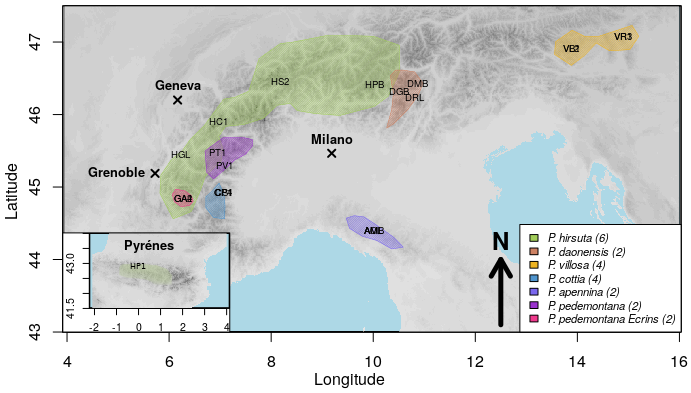
\includegraphics[width=1\textwidth]{fig/carte.png}
    \caption{\textbf{Carte de répartition de \textit{Primula} sect. \textit{Auricula} Duby subsect. \textit{Erythrodrosum} Pax.} Espèces composant la sous-section, avec entre parenthèse le nombre d'échantillons utilisés dans cette étude. Les aires de répartitions sont extrapolées depuis les observations de l'INPN et du CBNA. Les codes d'individus sur la carte reflètent le lieu d'échantillonnage. Fond de carte : Température moyenne annuelle extraite de WorldClim. Résolution 30s (1km$^{2}$).}
    %http://worldclim.org/version2
    \label{carte}
    \centering
\end{figure} 

La faible résolution phylogénétique obtenue jusqu'alors dans ce groupe étant probablement due à son origine récente \citep{Boucher2016} , la génétique des populations pourrait permettre d'éclairer le statut taxonomique de ces primevères. En effet, même si les données génétiques utilisées par \citet{Boucher2016a} ont été échantillonnées pour résoudre la phylogénie d'un groupe plus large, cette information sur tout le génome pourrait permettre d'estimer la structure génétique et les flux de gènes entre les populations des différents massifs alpins. Ces premières estimations sont également nécessaires pour orienter de futures campagnes d'échantillonnage et approfondir la connaissance de cette histoire biogéographique façonnée par les cycles glaciaires. 

Les objectifs de cette étude sont donc : (i) d'étudier la sous-section \textit{Erythrodrosum} à l'aide d'outils de génétique des populations; (ii) de clarifier la structure taxonomique de \textit{P. pedemontana s.l.}; (iii) de tester l'hypothèse d'admixture du taxon des Écrins.

%%%%% intro de flo %%%%%%
%Déterminer quelles entités taxonomiques constituent des espèces distinctes est un des objectifs premier de la taxonomie mais est également d’une importance primordiale pour comprendre à la fois l’origine des espèces, le processus de spéciation, et leur futur probable, qui détermine les mesures de conservation qui sont éventuellement à prendre pour les protéger.
%	Si délimiter des espèces vivant en sympatrie est généralement une tâche facile, les complexes d’espèces cryptiques ayant des distributions allopatriques présentent souvent plus de difficulté (Coyne & Orr 2004). En effet, dans ces derniers cas les critères qui servent généralement à établir la présence d’isolement reproductif (absence de flux de gènes ou  d’individus hybrides entre lignées, etc.) ne peuvent pas être mesurés objectivement (Fujita et al. 2012). Pourtant, délimiter des espèces cryptiques distribuées en allopatrie permet d’étudier le rôle d’un des mécanismes de spéciation majeurs : l’isolement géographique (Mayr 1942). Dans certains cas où la dynamique de l’environnement abiotique au cours du temps est bien connue, de telles études permettent même de caractériser précisément l’influence de l’environnement sur la divergence évolutive entre lignées (Avise et al. 1987).
%	Dans le cadre de ce stage, nous tenterons de comprendre comment la dynamique du relief dans les Alpes (i.e. les phénomènes d’orogénèse, d’érosion et de glaciation) a contribué à la divergence d’espèces au sein d’un groupe de plantes de haute montagne : Primula sect. Auricula Scott subsect. Erythrodrosum Pax (ci-dessous, clade Hirsuta). Ce groupe comprend traditionnellement six espèces proches de P. hirsuta All. mais une étude récente a proposé de re-circonscrire P. pedemontana en fusionnant trois espèces, tout en suggérant qu’un taxon distinct existe dans le massif des Ecrins en France (Boucher et al. 2016). Nos objectifs de recherche seront les suivants :
%	1) Reconstruire les relations phylogénétiques entre taxons du clade Hirsuta et dater leurs divergences
%	2) Délimiter les taxons qui méritent le rang d’espèce au sein de ce clade et en particulier au sein du complexe de P. pedemontana s.l.
%	3) Comparer statistiquement différents scénarios afin de comprendre comment la dynamique des reliefs Alpins a influencé la divergence des espèces du clade Hirsuta
%	Pour cela, nous utiliserons des données de séquençage haut-débit obtenues grâce à la technique hyRAD (Suchan et al. 2016) . Ces données comprennent plusieurs milliers de SNPs indépendants pour 22 individus appartenant aux six espèces du clade Hirsuta actuellement reconnues (Boucher et al. 2016). Nous les analyserons d’abord avec des approches phylogénétiques standard comme le logiciel RAxML (Stamatakis 2014) et des avancées nouvelles permettant de dater des phylogénies inférées grâce à des SNPs (Stange et al. 2018). Afin de délimiter des espèces le plus objectivement possible à l’aide des données moléculaires disponibles, nous utiliserons la panoplie variée des techniques de la taxonomie moléculaire, incluant des techniques de clustering génétique mais aussi d’autre basées sur le coalescent (Fujita et al. 2012, Carstens et al. 2013, Leaché et al. 2014). Enfin, nous aurons recours à l’inférence ABC pour comparer explicitement différents scénarios de spéciation (Knwoles 2009, Cornuet et al. 2014).
%	Cette étude devrait nous aider à mieux comprendre l’influence de la dynamique du relief sur l’évolution de la flore des Alpes. Elle permettra également d’établir plus fermement le statut taxonomique du nouveau taxon de Primula découvert dans le massif des Ecrins, qui reste à ce jour un mystère (http://www.ecrins-parcnational.fr/actualite/lenigme-de-la-primevere-du-valgaudemar), et éventuellement d’envisager des mesures de conservation.